The given  system of equations can be expressed in matrix form as 
\begin{align}
\myvec{3 & 1\\p & 2\\2 & -1} \vec{x} = \myvec{2\\3\\3}
\end{align}
%
Assuming the system of equations are consistent , lets reduce the augmented matrix to find the value of $p$
\begin{align}
    \myvec{3 & 1 & 2\\p & 2 & 3\\2 &-1 & 3} 
\xleftrightarrow {R_2\leftarrow R_2 -2 R_1} \myvec{3& 1 & 2\\P-6 & 0 & -1\\2 & -1 &3} 
\\
%\myvec{3 & 1 & 2 \\p-6 & 0 & -1\\0&-5&5}
\xleftrightarrow {R_3\leftarrow 3R_3 -2 R_1}\myvec{3 & 1 & 2 \\p-6 & 0 & -1\\0 & -5 & 5}
\\
%\myvec{3 & 1 & 2 \\p-6 & 0 & -1\\0&1&-1}
\xleftrightarrow {R_3\leftarrow -\frac{R_3}{5}}\myvec{3 & 1 & 2 \\p-6 & 0 & -1\\0 & 1& -1}
\end{align}
\begin{align}
 \myvec{3 & 1 & 2\\p-6 & 0 & -1\\0 & 1 & -1} 
\end{align}
%
Since the system of equations are assumed consistent, 
%
\begin{align}
 p-6 = -1
\\
\implies p = 5
\end{align}
Thus, the system of equations is given by 
\begin{align}
 \myvec{3 & 1}\vec{x}&=2 
\\
 \myvec{5 & 2 }\vec{x}&=3 
\\
 \myvec{2 & -1}\vec{x}&=3    
\end{align}
and plotted in Fig.     \ref{linform/20/fig:INTERSECTING LINES.}.
%
\begin{figure}[ht!]
    \centering
    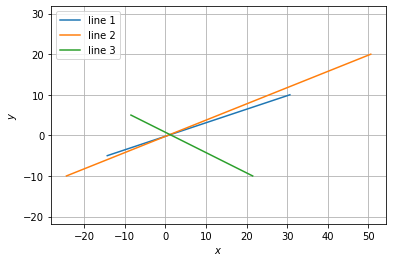
\includegraphics[width=\columnwidth]{solutions/su2021/2/20/FIG-4.png}
    \caption{INTERSECTING LINES.}
    \label{linform/20/fig:INTERSECTING LINES.}
\end{figure} 


